\documentclass[../piano-di-progetto.tex]{subfiles}

\begin{document}

\subsection{Analisi}
Il periodo di analisi inizia il 2020-03-09 con la formazione del gruppo e termina il giorno 2020-04-13 con la consegna dei documenti per la revisione dei requisiti. 

\subsubsection{Ruoli}
Durante questa macro, viene richiesta la presenza dei seguenti ruoli:
\begin{itemize}
    \item Responsabile;
    \item Amministratore;
    \item Analista;
    \item Verificatore.
\end{itemize}

\subsubsection{Attività}
Per semplicità, questa macro viene suddivisa in periodi:

\begin{itemize}

    \item \textbf{I periodo (2020-03-09 - 2020-03-16)}:
        \begin{itemize}
            \item \textbf{Discussione capitolati}: analisi e discussione dei capitolati proposti al fine di trovare gli aspetti positivi e negativi di ciascuno e individuare i capitolati di maggior interesse;
            \item \textbf{Ricerca degli strumenti}: ricerca degli strumenti di supporto da utilizzare durante le attività di progetto;
            \item \textbf{Normazione}: definizione delle \textsc{Norme di Progetto} per i processi di supporto e organizzativi;
            \item \textbf{Pianificazione attività e ruoli}: pianificazione e assegnazione delle attività preliminari;
            \item \textbf{Studio di fattibilità}: studio di tutti i capitolati;
            \item \textbf{Pianificazione della qualità}: definizione delle metriche per garantire la qualità di processo;
            \item \textbf{Verifica}.
        \end{itemize}
        \item \textbf{II periodo (2020-03-17 - 2020-03-24)}:
            \begin{itemize}
                \item \textbf{Verifica disponibilità proponenti}: le aziende proponenti vengono contattate per la conferma, o variazione, delle disponibilità dei capitolati;
                \item \textbf{Scelta capitolato}: decisione definitiva del capitolato da sviluppare;
                \item \textbf{Studio di fattibilità}: approfondimento dello \textsc{Studio di Fattibilità} del capitolato scelto;
                \item \textbf{Normazione}: definizione delle \textsc{Norme di Progetto} per i processi primari;
                \item \textbf{Pianificazione della qualità}: definizione delle metriche per garantire la qualità di prodotto;
                \item \textbf{Analisi dei rischi}: analisi approfondita dei rischi che il gruppo potrebbe riscontare durante lo svolgimento del progetto e definizione del relativo piano di contingenza;
                \item \textbf{Glossario}: aggiornamento del \textsc{Glossario};
                \item \textbf{Verifica}.
            \end{itemize}
        \item \textbf{III periodo (2020-03-25 - 2020-03-31)}:
        \begin{itemize}
            \item \textbf{Normazione}: completamento al dettaglio delle \textsc{Norme di Progetto};
            \item \textbf{Analisi dei casi d'uso};
            \item \textbf{Pianificazione delle attività}: pianificazione delle attività future e rispettivo preventivo;
            \item \textbf{Pianificazione della qualità}: specifica dei test;
            \item \textbf{Verifica}.
        \end{itemize}
        \item \textbf{IV periodo (2020-04-01 - 2020-04-08)}:
        \begin{itemize}
            \item \textbf{Analisi dei requisiti};
            \item \textbf{Resoconto}: stesura del consultivo di periodo e analisi dei rischi riscontrati;
            \item \textbf{Ricerca degli strumenti}: ricerca e studio autonomo degli strumenti richiesti dal proponente per lo sviluppo del progetto;
            \item \textbf{Glossario};
            \item \textbf{Verifica}.

        \end{itemize}

        \item \textbf{V periodo (2020-04-09 - 2020-04-11)}:
        \begin{itemize}
            \item \textbf{Stesura lettera di presentazione}: stesura della lettere di presentazione per la prima revisione di avanzamento;
            \item \textbf{Ricerca degli strumenti}: ricerca e studio autonomo degli strumenti richiesti dal proponente per lo sviluppo del progetto;
            \item \textbf{Consuntivo}: stesura del consuntivo di periodo;
            \item \textbf{Verifica}.
        \end{itemize}
    \end{itemize}

    \newpage
    \begin{landscape}
        \begin{figure}[H]
            \centering
            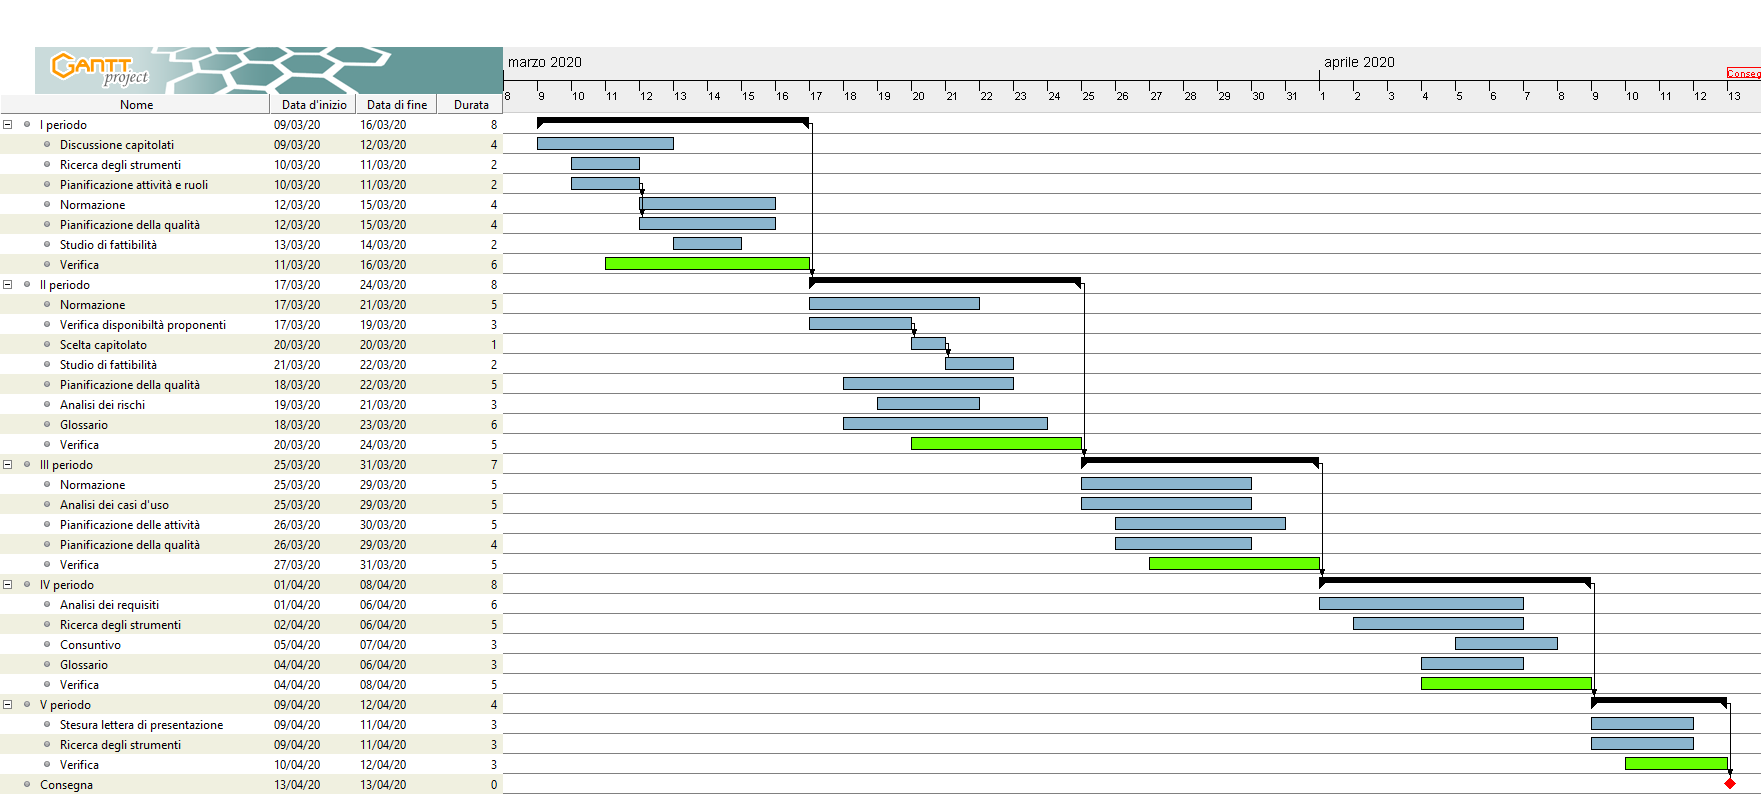
\includegraphics[width=24cm]{img/analisi.png}
            \caption{Diagramma attività nel periodo di analisi}
          \end{figure}
    \end{landscape}

\end{document}
